\documentclass{article}
\usepackage{tikz}
\usetikzlibrary{intersections}
\begin{document}
We are working on

\begin{tikzpicture}
  \draw (-1.5, 0) -- (1.5, 0);
  \draw (0, -1.5) -- (0, 1.5);
\end{tikzpicture}

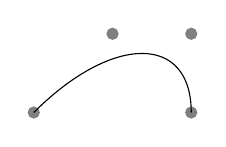
\begin{tikzpicture}
  \filldraw [gray] (0,0) circle [radius=2pt]
                   (1,1) circle [radius=2pt]
                   (2,1) circle [radius=2pt]
                   (2,0) circle [radius=2pt];
 \draw (0,0) .. controls (1,1) and (2,1) .. (2,0);
\end{tikzpicture}


\begin{tikzpicture}
  \draw (-1.5,0) -- (1.5,0);
  \draw (0,-1.5) -- (0,1.5);
  \draw (-1,0) .. controls (-1,0.555) and (-0.555,1) .. (0,1)
               .. controls (0.555,1) and (1,0.555) .. (1,0);
\end{tikzpicture}

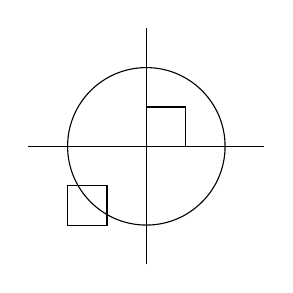
\begin{tikzpicture}
  \draw (-1.5, 0) -- (1.5, 0);
  \draw (0, -1.5) -- (0, 1.5);
  \draw (0, 0) circle [radius=1cm];
  \draw (0, 0) rectangle (0.5,0.5);
  \draw (-0.5,-0.5) rectangle(-1,-1);
\end{tikzpicture}

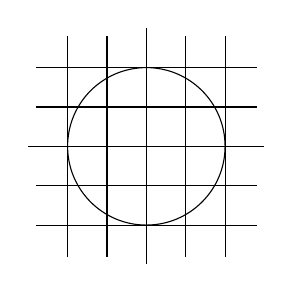
\begin{tikzpicture}
  \draw (-1.5,0) -- (1.5,0);
  \draw (0,-1.5) -- (0,1.5);
  \draw (0,0) circle [radius=1cm];
  \draw[step=.5cm] (-1.4,-1.4) grid (1.4,1.4);
\end{tikzpicture}

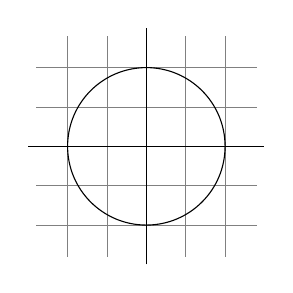
\begin{tikzpicture}
  \draw[step=.5cm,gray,very thin] (-1.4,-1.4) grid (1.4,1.4);
  \draw (-1.5,0) -- (1.5,0);
  \draw (0,-1.5) -- (0,1.5);
  \draw (0,0) circle [radius=1cm];
\end{tikzpicture}

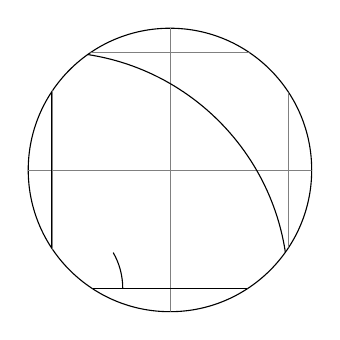
\begin{tikzpicture}[scale=3]
  \clip[draw] (0.5,0.5) circle (0.6);
  \draw[step=.5cm,gray,very thin] (-1.4,-1.4) grid (1.4,1.4);
  \draw (-1.5,0) -- (1.5,0);
  \draw (0,-1.5) -- (0,1.5);
  \draw (0,0) circle [radius=1cm];
  \draw (3mm,0mm) arc [start angle=0, end angle=30, radius=3mm];
\end{tikzpicture}

\tikz \draw (0,0) rectangle (1,1) (0,0) parabola (1,1);

\tikz \draw[x=1,y=1] (0,0) parabola bend (4,16) (6,12);

A sine \tikz \draw[x=1ex,y=1ex] (0,0) sin (1.57,2); curve.

\tikz \draw[x=1.57ex,y=1ex] (0,0) sin (1,1) cos (2,0) sin (3,-1) cos (4,0);

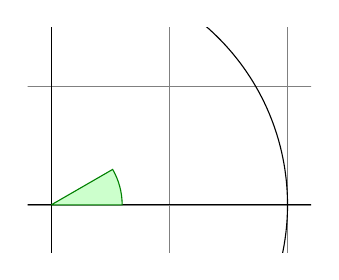
\begin{tikzpicture}[scale=3]
  \clip (-0.1,-0.2) rectangle (1.1,0.75);
  \draw[step=.5cm,gray,very thin] (-1.4,-1.4) grid (1.4,1.4);
  \draw (-1.5,0) -- (1.5,0);
  \draw (0,-1.5) -- (0,1.5);
  \draw (0,0) circle [radius=1cm];
  \fill[fill=green!20!white,draw=green!50!black] (0,0) -- (3mm,0mm)
    arc [start angle=0, end angle=30, radius=3mm] -- (0,0);
\end{tikzpicture}

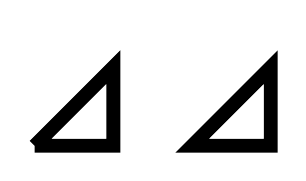
\begin{tikzpicture}[line width=5pt]
  \draw (0,0) -- (1,0) -- (1,1) -- (0,0);
  \draw (2,0) -- (3,0) -- (3,1) -- cycle;
  \useasboundingbox (0,1.5); % make bounding box higher
\end{tikzpicture}

\tikz \shade (0,0) rectangle (2,1) (3,0.5) circle (.5cm);


\begin{tikzpicture}[rounded corners,ultra thick]
  \shade[top color=yellow,bottom color=black] (0,0) rectangle +(2,1);
  \shade[left color=yellow,right color=black] (3,0) rectangle +(2,1);
  \shadedraw[inner color=yellow,outer color=black,draw=yellow] (6,0) rectangle +(2,1);
  \shade[ball color=green] (9,.5) circle (.5cm);
\end{tikzpicture}

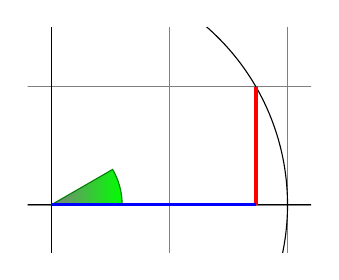
\begin{tikzpicture}[scale=3]
  \clip (-0.1,-0.2) rectangle (1.1,0.75);
  \draw[step=.5cm,gray,very thin] (-1.4,-1.4) grid (1.4,1.4);
  \draw (-1.5,0) -- (1.5,0);
  \draw (0,-1.5) -- (0,1.5);
  \draw (0,0) circle [radius=1cm];
  \shadedraw[left color=gray,right color=green, draw=green!50!black]
    (0,0) -- (3mm,0mm)
    arc [start angle=0, end angle=30, radius=3mm] -- cycle;
  \draw[red,very thick] (30:1cm) -- +(0,-0.5);
  \draw[blue,very thick] (30:1cm) ++(0,-.5) -- (0,0);
\end{tikzpicture}

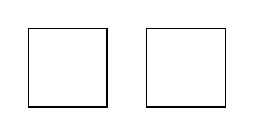
\begin{tikzpicture}
  \def\rectanglepath{-- ++(1cm,0cm)  -- ++(0cm,1cm)  -- ++(-1cm,0cm) -- cycle}
  \draw (0,0) \rectanglepath;
  \draw (1.5,0) \rectanglepath;
\end{tikzpicture}

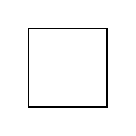
\begin{tikzpicture}
  \def\rectanglepath{-- +(1cm,0cm)  -- +(1cm,1cm)  -- +(0cm,1cm) -- cycle}
  \draw (0,0) \rectanglepath;
  % \draw (1.5,0) \rectanglepath;
\end{tikzpicture}

\tikz \draw (0,0) rectangle +(1,1)  (1.5,0) rectangle +(1,1);


% \begin{tikzpicture}
% \path [name path=upward line] (1,0) -- (1,1);
% \path [name path=sloped line] (0,0) -- (30:1.5cm); % a bit longer, so that there is an intersection
% % (add `\usetikzlibrary{intersections}' after loading tikz in the preamble)
% \draw [name intersections={of=upward line and sloped line, by=x}]
%   [very thick,orange] (1,0) -- (x);
% \end{tikzpicture}

\end{document}
